\documentclass[a4paper,12pt]{article}
\usepackage{graphicx}
\usepackage[left=30mm, right=30mm, top=30mm, bottom=30mm]{geometry}
\usepackage{amsmath}
\usepackage{siunitx}
\usepackage{fancyhdr}
\usepackage{url}
\pagestyle{fancy}
%-------------------------------------------------------------------------------
\lhead{\textbf{Spring 2019}}
\rhead{\textbf{CE394M Advanced Analysis in Geotechnical Engineering}}
\cfoot{\thepage}
%-------------------------------------------------------------------------------

\begin{document}
\begin{centering}
	\textbf{
		Assignment 6: Elastic parameters and Slope stability\\
		Assigned: 8th April 2019\\
		Due: 17th April 2019\\
	}
\end{centering}

\vspace{1em}
 
\begin{enumerate}

	\item A one-dimensional consolidation test, allowing no horizontal strain, was performed on a soil sample. At a vertical stress of 270 kPa, the vertical strain was measured as 0.2\% and the horizontal stress was measured as 115 kPa. From these results and assuming isotropic linear elasticity, develop two elastic parameters such that a complete \textbf{D} matrix can be specified for an analysis. Formulate the \textbf{D} matrix in both plane-stress and plane strain formulations.
	
	\item A consolidated-drained (CD) triaxial test is performed at an effective confining pressure of 100 kPa. A deviatoric stress of 20 kPa is applied. The resulting axial strain during the application of deviatoric stress is 0.08 \% and the resulting volumetric strain is 0.04\%. From these results and assuming isotropic linear elasticity, compute the radial strain and develop estimates of the shear modulus (G), bulk modulus (K), Poisson's ratio ($\nu$), and Young's modulus (E) of the soil.
	
	\item The stability of a sandy slope is a concern. The angle of the slope is 20 degrees. Since
	the length of the slope is long, it is assumed that it is infinitely long as shown in Fig. 1.
	The dry unit weight of the sand is $\gamma_d = 16 kN/m^3$, whereas the saturated unit weight is
	$\gamma_s = 18 kN/m^3$.
	
	A potential failure plane was found at 3 m depth as shown in Fig. 1. The peak friction angle of the sand at this location is 40 degrees. For the stability analysis of the infinite slope, forces acting on a soil block as shown in Fig. 1 are considered.
	
	\begin{enumerate}
		\item When the slope is completely dry, calculate the normal stress $\sigma$ and the shear stress $\tau$ acting at the base of the block. Is the slope likely to fail?
		\item Seepage is occurring parallel to the slope and the water table is at the slope surface as shown in Fig. 2. A standpipe piezometer is installed at Point A, which is located at a potential failure plane. Draw the equipotential lines and evaluate that the pore pressure at Point A.
		\item Using the pore pressure value obtained in part (b), calculate the effective normal
		and shear stresses acting at the base of the block. Is the slope likely to fail?
		\item Seepage is now occurring horizontally and the flow lines are shown in Fig. 3 and
		water is seeping out of the slope. Draw the equipotential lines and evaluate that the pore
		pressure at Point A.
		\item Using the pore pressure value obtained in part (d), calculate the effective normal
		and shear stresses acting at the base of the block. Is the slope likely to fail?
		\item If the slope is completely submerged into water and there is no seepage force, is the slope likely to fail? 
	\end{enumerate}

	\begin{figure}[!h]
		\centering
		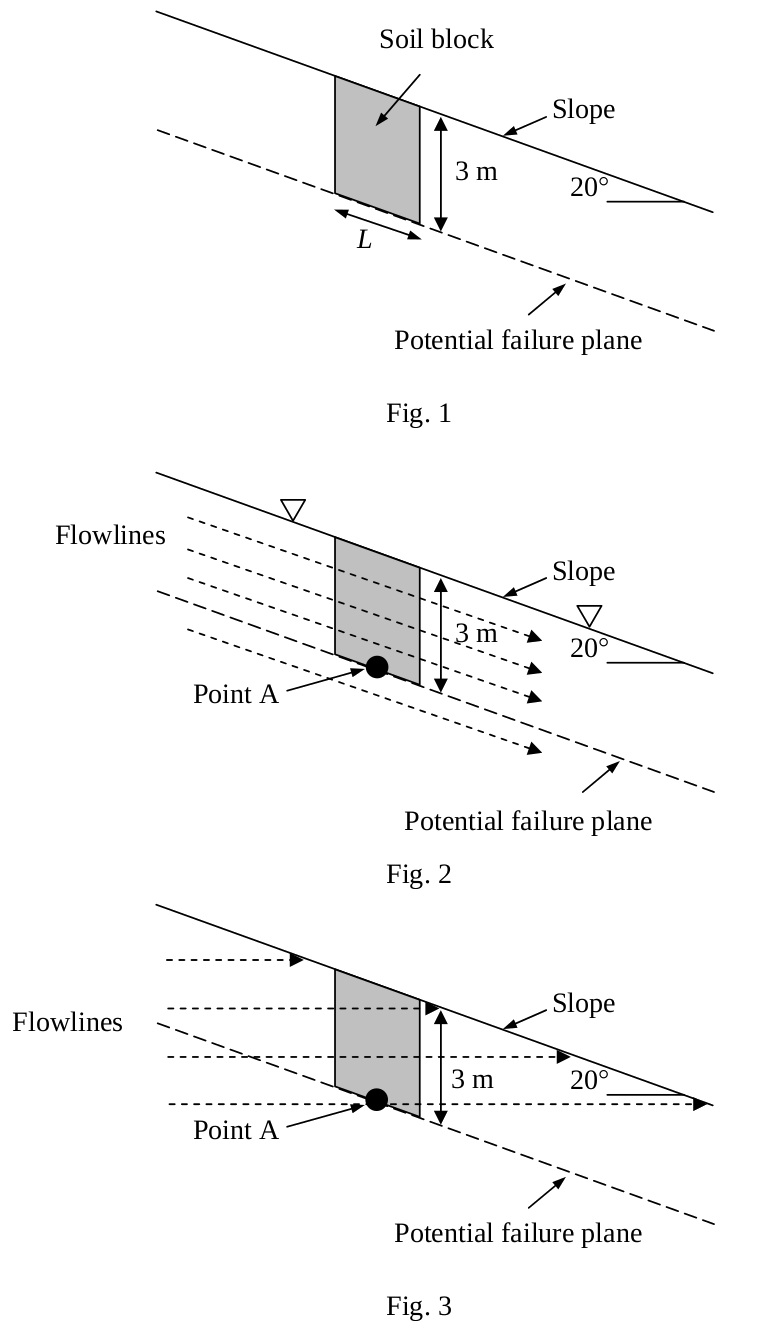
\includegraphics[width=0.65\textwidth]{figs/slopes.png}
	\end{figure}
	
	\item A long wide slope in glacial till with $\gamma = 20 kN/m^3$ and $\phi_{crit} = 25^o$ is to be cut to a slope angle of 18 degrees. The till forms a parallel layer about 5m deep and rests on top of a sloping impermeable bedrock. It is thought that the till has been overconsolidated to a vertical effective stress $\sigma_c^\prime = 250 kPa$, and that its monotonic peak shear strength
	envelope has the following relationship: $\tan \phi^\prime_{max} = \tan \phi^\prime_{crit} (\sigma_{crit}^\prime / \sigma^\prime)^{0.15}$. Surrounding slopes stream with water, and often fail.
	\begin{enumerate}
		\item Explain why the till may fail at its base.
		\item Are drains required to draw down the phreatic surface in order to ensure that the cut slope does not fail after the first wet season?
		\item Design the draw-down to ensure that the slope should never fail.
	\end{enumerate}
\end{enumerate}

\end{document}

